 \documentclass[11pt, oneside]{article}   	% use "amsart" instead of "article" for AMSLaTeX format
\usepackage{geometry}                		% See geometry.pdf to learn the layout options. There are lots.
\geometry{letterpaper}                   		% ... or a4paper or a5paper or ... 
%\geometry{landscape}                		% Activate for for rotated page geometry
%\usepackage[parfill]{parskip}    		% Activate to begin paragraphs with an empty line rather than an indent
\usepackage{graphicx}				% Use pdf, png, jpg, or eps§ with pdflatex; use eps in DVI mode
								% TeX will automatically convert eps --> pdf in pdflatex		
\usepackage{amssymb}
\usepackage{amsmath}
\usepackage{parskip}
\usepackage{color}
\usepackage{hyperref}

\title{Residue Theory 1}
%\author{The Author}
%\section{}
%\subsection*{}
\date{}							% Activate to display a given date or no date

\graphicspath{{/Users/telliott_admin/Dropbox/Tex/png/}}
% \begin{center} 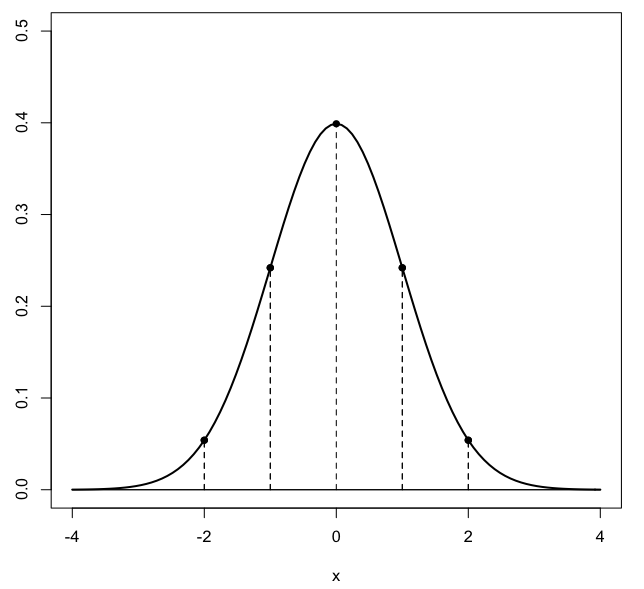
\includegraphics [scale=0.4] {gauss3.png} \end{center}
\begin{document}
\maketitle
\Large
If I'm understanding correctly, a sketch of the road ahead looks like this.  Cauchy's theorem says that the integral around a closed path for an analytic function is zero.  If such a function is undefined at a limited number of points (because it is a fraction with zero in the denominator), then those points are called poles or singularities and Cauchy 2 can be used to calculate the value of the integral (called a residue) from the value of the function at those points.

All complex functions can be expanded as power series around a fixed point $z_0$.  This isn't always useful, like if the radius of convergence $R = 0$, but otherwise it is.  Unlike with Taylor series, these Laurent series contain terms with negative powers.  So, when integrating a function by integrating its series, we obtain a bunch of terms in different integral powers of $(z-z_0)^n$.

But by the reasoning we've given, only the term with $(z-z_0)^{-1}$ has a non-zero integral.

Let's look at some examples of integrals like this, starting with one we've done before.
\[ \int \frac{1}{z} \ dz \]
We can do this one in terms of $x$ and $y$, but $r e^{i \theta}$ is a little easier.  The answer will be the same.

We parametrize a circle of radius $r$ centered on the origin:
\[ z(t) = r e^{it} \]
We have that $z'(t)$ is
\[ \frac{dz}{dt} = i r e^{it} = i z \]
so
\[ dz = i z \ dt \]

In general, if write a parameterized formula for a curve:
\[ z(t) = x(t) + iy(t) \]
Then the integral is
\[ \int z(t) \ dz = \int z(t) z'(t) \ dt \]

Now for this particular problem, we have
\[ I = \int \frac{1}{z} \ dz \]
and we plug in 
\[ dz = i z \ dt \]
\[ I = \int \frac{1}{z} \ i z \ dt \]
The $z$ on top and bottom cancel and we're left with
\[ I = \int i \ dt \]
\[ = i \int dt \]
For a closed path, this integral is equal to $2 \pi$ so the final answer is 
\[ I = 2 \pi i \]
The result is seen to be independent of the radius of the circle.

\subsection*{translated from the origin}
Suppose we are interested in the value of the integral centered at a point $z_0 \ne 0$.  We consider those points $z$ in a circle constructed around $z_0$, that is
\[ z = z_0 + re^{it} \]
rearranging
\[ z - z_0 = re^{it} \]
We get the derivative of the polar form
\[ \frac{d}{dt} \ re^{it} = i re^{it}  \]
\[ = i(z-z_0) \]
Hence
\[ \int \frac{1}{(z-z_0)} \ dz  = \int \frac{1}{(z-z_0)} \ i(z - z_0) \ dt \]
\[ = 2 \pi i \]

[ I'm a little confused about why this goes off the rails.  Since $z_0$ is a constant:
\[ \frac{d}{dt} \ [ \  z - z_0  \ ] \ =   \frac{d}{dt} \  z = \frac{dz}{dt}  \]
?? ]

However, we can also do this by Cauchy 2. The formula is
\[ \int \frac{f(z)}{z - z_0} \ dz = 2 \pi i \ f(z_0) \]
here the integrand is
\[ \frac{1}{(z-z_0)} \]
so $f(z)$ is just equal to $1$, and the answer is $2 \pi i$.

\subsection*{problem}
Let's try one with something a bit more complicated in the denominator.  This problem is Beck 4.26.  Consider 
\[ f(z) = \frac{1}{z^2 + 1} \]
What is $\int f(z) \ dz$ ?  We see that the denominator is zero when
\[ z^2 = -1 \]
\[ z = \pm \ i \]
Furthermore we can factor
\[ z^2 + 1 = (z + i) (z-i) \]
and we see the same result, that this is zero when $z = \pm \ i $.

Now, suppose the curve is the unit circle centered at $i$, designated as $C[i,1]$.  Obviously, this curve contains the singularity $z = i$.  The curve goes through the origin, so it does not extend as far as $z = -i$.

Rewrite the function as
\[ f(z) = \frac{1/z+i}{z-i} \]
Thus
\[ \int \frac{1}{z^2 + 1} \ dz = \int \frac{1/z+i}{z-i} \ dz \]

Cauchy's Integral formula says that
\[ f(z_0) = \frac{1}{2 \pi i} \ \oint  \frac{f(z)}{z-z_0} \ dz \]
or equivalently
\[ 2 \pi i \ f(z_0) = \oint  \frac{f(z)}{z-z_0} \ dz \]

The function is
\[ \frac{1}{z+i} \]
and when evaluated at $i$, with result $1/2i$, we obtain
\[ \oint  \frac{f(z)}{z-z_0} \ dz = 2 \pi i \ f(z_0) \]
\[ = 2 \pi i \ \frac{1}{2i} = \pi \]

Similarly, if the unit circle had been centered at $-i$, rewrite the function as
\[ f(z) = \frac{1/z-i}{z+i} \]
The value of the function is
\[ \frac{1}{z-i}(-i) = -\frac{1}{2i} \]
and that integral is then $- \pi$.

A contour that includes both singularities integrates to zero.
\subsection*{partial fractions}
We can also do the curve containing both singularities by partial fractions.  Write
\[ \frac{1}{z^2 + 1} = \frac{1}{(z+i)(z-i)} \]
\[ = \frac{A}{z+i} + \frac{B}{z-i} \]
We need to determine $A$ and $B$.  When we multiply to put everything over the common denominator ($z^2 + 1)$ then for the numerators we will have:
\[ A(z-i) + B(z+i) = 1 \]
This gives
\[ Az + Bz = 0 \]
Hence $A = -B$.  And
\[ -Ai + Bi = 1 \]
\[ -Ai - Ai = -2Ai = 1 \]
\[ A = -\frac{1}{2i} \]
Hence the integrand is
\[ \frac{1}{z^2 + 1} = = \frac{A}{z+i} + \frac{B}{z-i} \]
\[ = -\frac{1}{2i(z+i)} + \frac{1}{2i(z-i)} \] 
For the curve including $z = i$ but not $z = -i$ we have that the left-hand integral is 0 by Cauchy's Theorem, and for the right hand side the function is
\[ f(z = z_0) = \frac{1}{2i} \]
So the value of the integral is
\[ 2 \pi i f(z_0) = 2 \pi i \ \frac{1}{2i} = \pi \]
as before.  The other pole we would have
\[ f(z = z_0) = -\frac{1}{2i} \]
and the result would be $- \pi$.  A curve enclosing both poles would have integral equal to zero.

\subsection*{connection to the real numbers}
Note the corresponding real function
\[ \int_0^{\infty} \frac{1}{1 + x^2} \ dx \]
We know the answer to this one, it is 
\[ \tan^{-1} x \ \bigg |_0^{\infty} = \frac{\pi}{2}  \]
Since $f(x)$ is an even function, the integral over $-\infty \rightarrow \infty = \pi$.

We feel there ought to be a connection between the two results:  real and complex.

Suppose we draw a different curve (contour) extending on its base from $-\infty \rightarrow \infty$: the real axis.  That integral is $\int f(z) \ dz$ but $y$ and $dy$ are both zero so it becomes just $\int f(x) \ dx$ with the result shown.

How to complete the contour?  Imagine a semicircle in the upper half-plane with $R \rightarrow \infty$.  That is, parametrize
\[ \gamma(\theta) = Re^{i\theta}, \ \ \ \theta \in [0, \pi] \]
\[ \gamma \ '(\theta) =  iRe^{i\theta} \]
The integral is
\[ \int_0^{\pi} \frac{1}{1 + R^2 e^{i2\theta}} \ i R e^{i \theta} \ d \theta \]
Now what?

We'll try to be more formal later, but just for now, it's clear that as $R \rightarrow \infty$, this integrand goes to 0.  So we have that the total integral for the complex case is equal to the integral for the real part plus this extra half-circle which is zero.

What this means is that if we had not know the result for the real integral, we could deduce it from the fact that the whole complex integral has value equal to $\pi$, and the part over this complex half-circle is zero.

\subsection*{another problem}

Consider
\[ \int_{\gamma} \frac{z^2}{4-z^2} \ dz \]
where $\gamma = | z + 1 | = 2$.
So the denominator of the function is
\[ \frac{1}{4-z^2} = \frac{1}{(2+z)(2-z)} \]
It has zeroes as $z = \pm \ 2$.  Only the point $z = 2$ is inside our contour.  So if we split this by partial fractions
\[  \frac{1}{(2+z)(2-z)} = \frac{1}{4} \ [ \ \frac{1}{2+z} + \frac{1}{2-z} \ ] \]
so we can rewrite the integral as
\[ I = \int_{\gamma} \frac{z^2}{4} \ [ \ \frac{1}{2+z} + \frac{1}{2-z} \ ] \ dz \]

By Cauchy's Theorem, the first term is zero.  The second one is:
\[ I = \int_{\gamma} \frac{z^2}{4} \ ( \frac{1}{2-z} ) \ dz \]
and the value of $I$ is
\[ I = 2 \pi i f(z_0) \]
where 
\[ f(z_0) = \frac{z^2}{4}  \ \bigg |_{z_0 = 2} = 1 \]
so the integral is just $2 \pi i$.

\subsection*{one from wikipedia}
Consider
\[ g(z) = \frac{z^2}{z^2 + 2z + 2} \]
We want to evaluate the integral:
\[ I = \oint g(z) \ dz \]

The denominator
\[ z^2 + 2z + 2 \]
can be factored.

We plug into the quadratic solution:
\[ \frac{-b \pm \sqrt{b^2 - 4ac}}{2a} =  \frac{-2 \pm \sqrt{4 - 4 \cdot 2}}{2} \]
\[ = -1 \pm \  \frac{\sqrt{-4}}{2} \]
\[ = -1 \pm i \]
The zeroes of the denominator are
\[ - 1 + i \ , \ \ \ - 1 - i \]
From this we construct the two factors as
\[ z - (- 1 + i) = z + 1 - i \]
\[ z - (-1 - i) = z + 1 + i \]

We confirm that these two factors multiplied together give back what we started with:
\[ (z + 1 + i) \ (z + 1 - i) \]
\[ = z^2 + z + iz + z + 1 + i + -iz - i + 1 \] 
\[ = z^2 + 2z + 2 \]

So we can factor the denominator and write:
\[ \frac{1}{z^2 + 2z + 2} = \frac{A}{z + 1 - i} + \frac{B}{z + 1 + i}  \]
Putting these two terms over a common denominator means multiplying the two factors and restoring what we started with.

For the numerator we have
\[ A(z + 1 + i) + B(z + 1 - i) = 1 \]
\[ Az + A + iA + Bz + B - iB = 1 \]
Equating terms containing the same power of $z$ gives two simultaneous equations:
\[ Az + Bz = 0z \]
and
\[ A(1 + i) + B(1 - i) = 1 \]

So $A = -B$ and
\[ A(1 + i) + B(1 - i) = 1 \]
\[ A (1 + i) - A(1 - i) = 1 \]
\[ A 2i = 1 \]
\[ A = \frac{1}{2i}, \ \ \ B = -\frac{1}{2i} \]
The integral is
\[ \oint z^2 \ [ \ \frac{1}{2i} \ \frac{1}{z + (1 - i)} - \frac{1}{2i} \ \frac{1}{z + (1 + i)} \ ] \ dz \]
\[ = \frac{1}{2i} \ [ \ \oint \frac{z^2}{z + (1 - i)} \ dz - \oint \frac{z^2}{z + (1 + i)} \ dz \ ] \]

So we see that we have a sum of integrals of the form
\[ \oint \frac{f(z)}{z - z_0} \]
The residues occur at the points
\[ z = z_0 \]
that is at 
\[ z = - (1 - i) = -1 + i \]
\[ z = - (1 + i) = -1 - i \]

If the contour is $|z| = 2$ centered at the origin (the circle of radius $2$, then both of the points lie within the contour.  ($ r^2 = 2$ for both).

We evaluate $2 \pi i f(z_0)$ for each
\[ f(z) = z^2 \]
The first term gives
\[ f(z_0) = (-1 + i)^2 =  -1 -1 - 2i \]
The second term gives 
\[ (-1 -i)^2 = -1 - 1 + 2i \]
Each of these needs to be multiplied by $2 \pi i$.

Go back and see that we had the sum of the first term plus the negative of the second term, all multiplied by $1/2i$
\[ \frac{1}{2i} \ [ \ 2 \pi i (-1 -1 - 2i) - 2 \pi i (-1 - 1 + 2i) \]
\[ = \pi \ [ (-1 -1 - 2i) -  (-1 - 1 + 2i) \ ] \]
\[ = -4 \pi i \]

\end{document}  